\documentclass[a4paper]{article}

% Pacotes para o português.
\usepackage[brazilian]{babel}
\usepackage[utf8]{inputenc}
\usepackage[T1]{fontenc}

\usepackage{sbc-template}

\usepackage{datetime}
\usepackage{graphicx}
\usepackage{float}
\usepackage{indentfirst}
\usepackage{amssymb}
\usepackage{multirow}
\usepackage[nottoc]{tocbibind}

% Espaçamento duplo.
\usepackage{setspace}
 % Breaklines nas citações.
\usepackage{cite}

% Linha horizontal.
\newcommand{\HRule}{\rule{\linewidth}{0.5mm}}
\newcommand{\hRule}{\rule{4.5cm}{0.1mm}}

% Listagens.
\newfloat{program}{thp}{lop}
\floatname{program}{Listagem}

% Figuras.
\newcommand{\figurex}[5]
{
\begin{figure}[htb, h!]
   	\setlength{\unitlength}{1.0cm}
   	\centering
   	\includegraphics[scale=#1]{./img/#2.#3}
	\begin{center}
	   	\parbox{.9\linewidth}{\footnotesize \sf \caption{#5}  \label{#4}}
	\end{center}
\end{figure}
}

\newcommand{\ck}[0]
{
\checkmark
}

\hyphenation{}

\begin{document}

%\doublespacing
\onehalfspacing

\begin{titlepage}
\begin{center}

% Topo 1.
\textsc{\Large UNIVERSIDADE FEDERAL DE ITAJUBÁ\\
	INSTITUTO DE MATEMÁTICA E COMPUTAÇÃO}\\[0.7cm]

% Topo 2.
\textsc{DEPARTAMENTO DE MATEMÁTICA E COMPUTAÇÃO}\\[2.8cm]

% Título.
\textsc{\Large Seminário}\\
\HRule \\[0.4cm]
{\Large \bfseries Arquitetura Peer to Peer}
\HRule \\[0.4cm]
\textsc{REDES DE COMPUTADORES}\\[2.8cm]

% Etc.
\begin{minipage}{0.4\textwidth}
\begin{flushleft} \large
\emph{Alunos:}\\[0.43cm]
%\hRule\\
David Mateus Batista\\
Gabriel Erzinger Dousseau\\
Gabriel Augusto Alves Taets\\
Maurício Leite Ferreira\\
\end{flushleft}
\end{minipage}
\begin{minipage}{0.4\textwidth}
\begin{flushright} \large
\emph{Professor:}\\[0.4cm]
%\hRule\\
Bruno Guazzelli Batista
\end{flushright}
\end{minipage}

\vfill

\today

\end{center}
\end{titlepage}

\thispagestyle{empty}

\section*{Resumo}
Esta monografia tem o objetivo de estudar e analisar a arquitetura de redes Peer-to-peer,
suas vantagens, desvantagens, limitações e aplicações.
\newpage
\pagenumbering{Roman}

\tableofcontents
\newpage
\pagenumbering{arabic}

%http://www.fio.edu.br/manualtcc/co/1_Estrutura_do_TCC.html%
\section{Introdução}
\newpage

\section{Fundamentação Teórica}
\textit{Peer-to-Peer} significa, em tradução literal, "par a par". Em termos formais, os dispositivos da rede estão conectados por uma cadeia descentralizada, onde cada um possui funções equivalentes, sem hierarquias. Todos os usuários são clientes e servidores, funcionando de forma independente e livre da existência de um servidor central. A busca por um arquivo é enviada a todos os dispositivos da rede, os quais tomam conhecimentos dos outros usuários através de um hospedeiro (que apenas monitora pontos de presença na rede e não tem um banco de dados com nomes de usuários ou arquivos), que informa o IP dos usuários ativos na rede. O pedido é repassado para todos os usuários, que vão passando, usuário por usuário, até que o arquivo desejado seja encontrado.\cite{sisp2p}

É preciso notar que P2P e arquiteturas centralizadas não são alternativas disjuntas. Existem muitos sistemas que podem ser classificados como uma mistura de um sistema P2P e um sistema centralizado. O problema é que não existe uma fronteira clara entre um paradigma P2P e outros paradigmas supostamente opostos como cliente-servidor. Nos extremos, algumas arquiteturas são claramente P2P enquanto outras são claramente cliente-servidor. No entanto, existem arquiteturas que podem ser consideradas uma ou outra ou ambos, dependendo da definição de P2P considerada. Consequentemente, é importante entender o que é comum a todas as definições de P2P e o que são traços não-comuns que alguns autores incluem em suas próprias definições.\cite{camarillop2parch}

Considera-se um sistema P2P se os elementos que formam o sistema compartilham seus recursos com o propósito de prover o serviço que o sistema foi desenhado para prover. Os elementos no sistema tanto proveem os serviços aos outros elementos, como requisitam os serviços aos outros elementos. A princípio, todos os elementos no sistema devem satisfazer este critério para que o sistema seja considerado P2P. No entanto, na prática, o sistema pode ter algumas exceções (isto é, alguns nós que não satisfazem este critério) e ainda ser considerado P2P. Por exemplo, um sistema P2P pode ainda ser considerado P2P mesmo se tiver um servidor centralizado de registros. Por outro lado, alguns sistemas dividem \textit{endpoints} entre pares e clientes. Pares requisitam e oferecem serviços, enquanto clientes geralmente apenas requisitam serviços. Um sistema onde a maioria dos \textit{endpoints} se comportam como clientes não pode ser considerado estritamente P2P. \cite{camarillop2parch}

Alguns autores adicionam ainda que os elementos que formam os sistemas P2P (que não surpreendentemente são denominados \textit{pares}), devem ser capazes de se comunicarem diretamente, sem passar por intermediários \cite{schollmeier2001}. Outros autores dizem que o sistema deve ser auto-organizável e ter controle decentralizado\cite{roussopoulos2004}.

É notável que as definições acima são dadas no contexto de um único serviço individual. Um serviço complexo pode ser composto de vários serviços individuais. Alguns desses serviços individuais pode consistir de serviços P2P e alguns deles podem consistir de serviços cliente-servidor. Por exemplo, um cliente de compartilhamento de arquivos pode incluir um cliente P2P para efetuar o compartilhamento em si, e um navegador \textit{web} para acessar informações adicionais num servidor \textit{web} centralizado. Adicionalmente, existem arquiteturas onde um sistema cliente-servidor pode servir como "estepe" para um serviço normalmente provido por um sistema P2P, ou vice-versa. \cite{camarillop2parch}

Prover um serviço geralmente envolve processamento ou armazenamento de dados. De acordo com a definição de Camarillo, num sistema P2P, os pares compartilham suas capacidades de processamento e armazenamento (isto é, seus recursos de software e hardware), de forma que o sistema possa prover o serviço. Por exemplo, se o serviço a ser provido é um serivço de distribuição de arquivos, pares diferentes entre o sistema irão armazenar arquivos diferentes. Quando um certo par quer um arquivo em particular, primeiro ele deve descobrir qual par possui (ou quais pares possuem) o arquivo, e então obter o arquivo destes pares\cite{camarillop2parch}. Esta definição de P2P nos fornece um critério para decidir se um sistema é ou não P2P.


\begin{figure}[!hb]
\begin{center}
  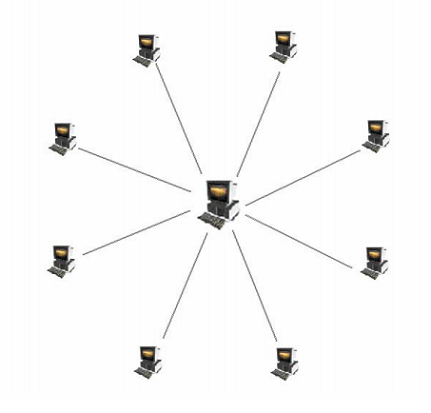
\includegraphics{img//cliente-servidor.png}
  \caption{Esquema Cliente-Servidor\cite{sisp2p}} 
\end{center}
\end{figure}
A imagem acima representa um sistema cliente-servidor, onde o nó central é o servidor, e ele responde as requisições de todos os clientes.

\begin{figure} [!ht]
\begin{center}
  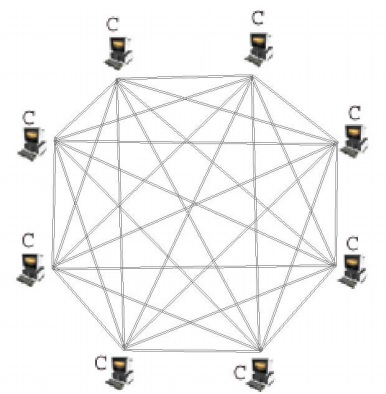
\includegraphics{img//p2p.png}
  \caption{Esquema P2P \cite{sisp2p}} 
\end{center}
\end{figure}
A imagem acima representa um sistema P2P, onde todos os nós são ligados a todos os nós, e as requisições podem ser feitas e respondidas por qualquer nó.

\begin{figure} [!ht]
\begin{center}
  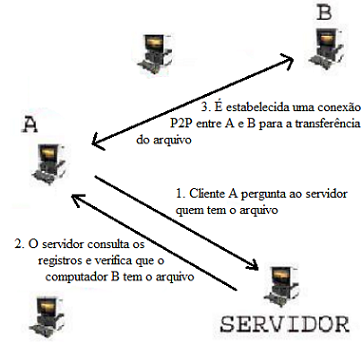
\includegraphics{img//misto.png}
  \caption{Esquema Misto \cite{sisp2p}} 
\end{center}
\end{figure}
A imagem acima representa um esquema misto, onde existe um servidor centralizado que recebe as requisições e direciona a requisição para um nó que possa respondê-la.

\newpage

\section{Aplicações}
Como visto nas seções anteriores, a utilização da arquitetura \textbf{P2P} pode trazer diversas vantagens, desvantagens e outras características únicas para o aplicativo ( ou serviço ) que estará implementando-a. 

Dessa forma, é importante analisar quais serviços utilizam essa arquitetura, como se beneficiam de suas vantagens e como lidam com suas desvantagens. Isto é, dissecar sobre como as características da arquitetura P2P são tratadas em cada caso de uso.
\subsection{Napster}
O \textbf{Napster} foi uma das primeiras aplicações de compartilhamento de arquivos, elaborada em Junho de 1999. O serviço permitia apenas o compartilhamento de arquivos \textbf{MP3} e é um grande responsável pela popularidade do termo "P2P".

A rede se baseia num servidor central de índices. Os nós da rede registram uma lista dos arquivos que desejam compartilhar. Dessa forma, a busca é processada baseando-se em \textbf{palavras chave} e retornará uma lista com os arquivos encontrados e informações como a banda disponível, tamanho e fonte. 

\begin{figure}[!h]
\begin{center}
  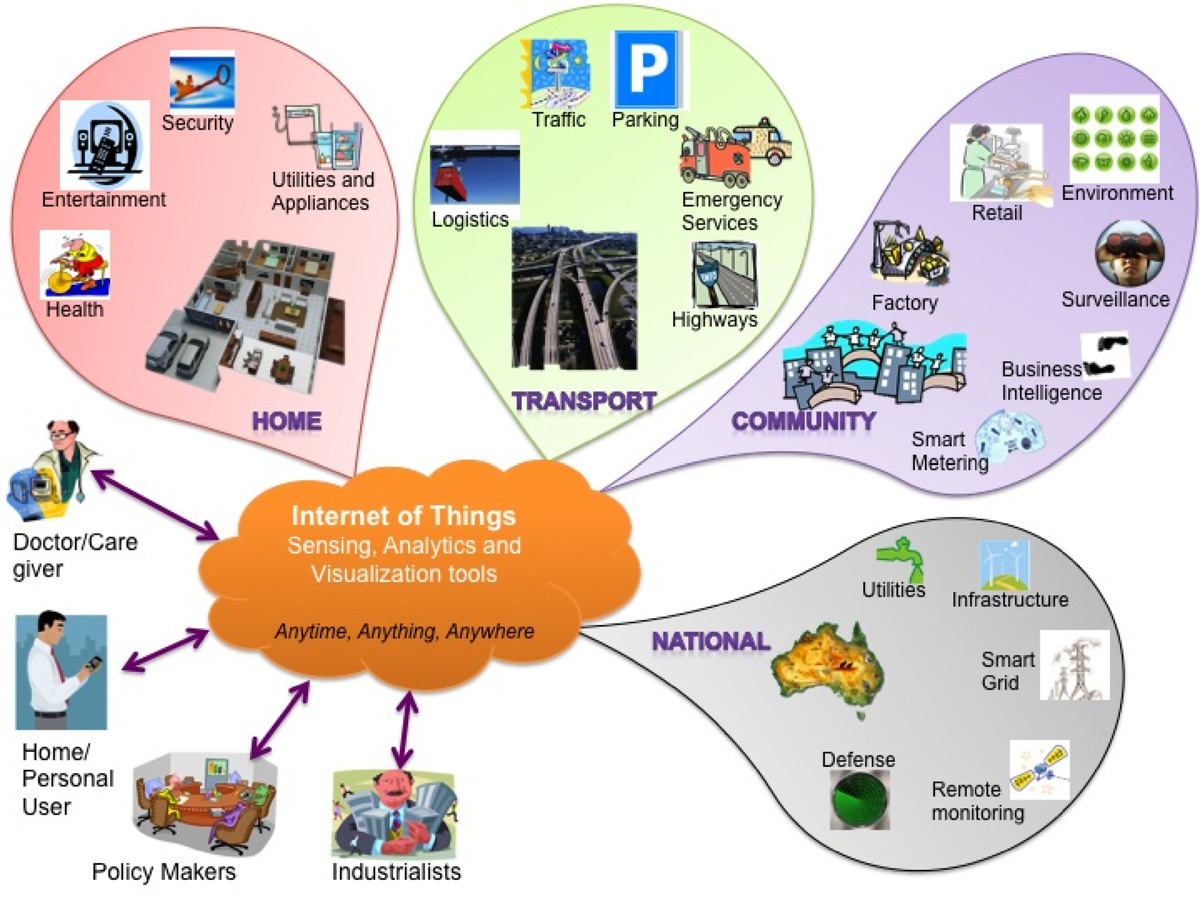
\includegraphics{img//ilustracaoiot.png} 
  \caption{Protocolo Napster \cite{howstuffworks} \label{figure1}}
\end{center}
\end{figure}

A imagem acima representa o funcionamento do protocolo Napster, indicando um cliente fazendo uma \textbf{consulta} ao servidor central, para que o servidor então busque os outros clientes que possuem tal arquivo. Em seguida, tais clientes se conectam ao requisitante, para transferir o arquivo.

\subsubsection{Vantagens e Desvantagens}
Como um dos pioneiros na área, a principal vantagem do Napster se devia ao fato de ele possuir uma busca rápida e eficiente ( por se tratar apenas de uma consulta ao servidor central ). Além disso, oferecia uma visão simples e consistente da rede. 

As desvantagens se devem exatamente a \textbf{presença de um servidor}, uma vez que, assim como em arquiteturas cliente-servidor, a central representa um ponto de falha único, que se fosse afetado, prejudicaria toda a rede. Por se tratar de um servidor que lida com diversas requisições, o servidor central também possuía um alto custo de manutenção.
\subsection{Gnutella} %https://pdfs.semanticscholar.org/f0b5/86bda8901c2f3ae399b48239690028f69417.pdf
%https://pt.slideshare.net/uschmidt/peertopeer-systems/7-P2P_Filesharing_The_most_popular
Gnutella é um \textbf{protocolo de busca} aberto e descentralizado usado principalmente para o compartilhamento e a busca de arquivos. Foi criado com o objetivo de ser uma rede dinamica que permite que seus usuários entrem e saiam a qualquer momento, tenha uma boa escalabilidade, garanta a anonimidade  e confiança em relação a ataques externos.\cite{gayatriGN}

O termo Gnutella se refere a todo o grupo de computadores que possuem aplicativos carregados com o protocolo Gnutella que formam uma espécie de rede virtual. Cada nó nessa rede pode funcionar tanto como um cliente como quanto um servidor. 

Dessa forma, eles podem criar e receber requisições com outros nós utilizando os dados que estarão em seu disco rígido. Como é sabido, tais requisições não são enviados para nenhum servidor central, elas são exclusivamente tratadas entre os nós da rede. 

\begin{figure}[!h]
\begin{center}
  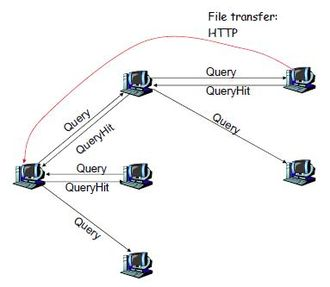
\includegraphics{img//gnuquery.JPG} 
  \caption{Protocolo Gnutella \cite{examplesofp2p} \label{figure1}}
\end{center}
\end{figure}


A imagem acima, representa um grupo de computadores utilizando aplicativos com o protocolo Gnutella. Na mesma, um computador realiza uma \textbf{query} buscando um arquivo nos nós da rede. Os computadores que possuírem tal arquivo, retornam um \textbf{Query hit} para que, em seguida, seja estabelecida uma conexão \textbf{HTTP} entre eles para a transmissão do arquivo. 



\subsubsection{Mecanismo de Busca}
O protocolo utiliza o algoritmo padrão conhecido como BFS( \textbf{B}readth \textbf{F}irst \textbf{S}earch) - Busca em Largura - portanto, tal qual o algoritmo é utilizado em grafos, ele será utilizado na rede de aplicativos que utilizam o protocolo:\cite{gayatriGN}
\begin{itemize}
	\item O nó inicialmente busca um arquivo e envia a mensagem de busca a seus vizinhos
	\item Os vizinhos encaminham a mensagem para todos os seus vizinhos
	\item Os Nós que possuírem o arquivo que está sendo requisitado, começam uma mensagem de resposta
	item. Após a mensagem de resposta atingir o nó origem, o download do arquivo começa.
\end{itemize}
\subsubsection{Vantagens e Desvantagens}
O protocolo GNutella apresenta algumas modificações que \textbf{superam} as desvantagens do Napster, como por exemplo: não depender de um servidor para indexar os arquivos, dessa forma, não se cria um "único ponto de falha" na arquitetura. Entretanto, este mesmo fato causa uma das suas principais desvantagens: a busca em largura acaba por adicionar um certo período de tempo bem maior do que se fosse utilizado um servidor.

Além disso, outros pontos de falha do protocolo Gnutella são: o fato de que metade dos arquivos são servidos por apenas 1 porcento dos usuário , além da perca de banda larga e segurança em relação a transmissão de arquivos mascarados.\cite{gayatriGN}

\subsection{BitTorrent}
Apesar de muitos sistemas de compartilhamento de arquivos terem sido propostos e implementados, poucos persistirão ao teste intensivo de uma grande quantidade de usuários diários. O \textbf{BitTorrent} é um destes sistemas que, além de persistir, evoluiu como uma das mais populares redes da internet. De fato, a pesquisa \textbf{The True Picture of Peer-to-Peer File sharing} indica que, em Junho de 2004, o sistema era responsável por mais da metade de todo o tráfico P2P do mundo. \cite{pouwelsebit}. Dessa forma, nesta monografia, citamos o sistema BitTorrent como representante das demais aplicações de torrents que funcionam de forma parecida, porém que não alcancaram o a mesma difusão e boa performance.

Diferente do que visto anteriormente, o BitTorrent é apenas um protocolo de download de arquivos, de forma que dependa de outros serviços ou websites para fazer a busca destes arquivos\cite{pouwelsebit, CohenBIT}.

\subsubsection{Funcionamento}

O sistema funciona dividindo um arquivo em partes menores, dessa forma, ao se executar o download do arquivo, o usúario ao mesmo tempo realiza o upload de uma \textbf{parte} do arquivo que ele já possui, para outros usúarios que ainda não possuem esta parte. Todo este funcionamento é gerenciado de forma a otimizar a taxa de download e upload. 

Um usuário com uma alta taxa de upload, tem uma chance maior de possuir também uma alta taxa de download, o que funciona como um incentivo para que os usúarios contribuam com a rede. Quando um usúario finaliza o download de um arquivo, ele permanece como uma semente, executando apenas o upload deste arquivo, para colaborar com a rede. \cite{CohenBIT}

Para se publicar um arquivo utilizando tal sistema, primeiro um arquivo estatico $.torrent$ é adicionado a qualquer servidor web para que os usuários o encontrem. Este arquivo contem informações como o tamanho, nome, hash e a url de um $tracker$.  Estes trackers são responsáveis por fazer com que os usúarios da rede se ``encontrem''.  Para dar inicio, basta então, que um usúario que contenha o arquivo em sua totalidade inicie o arquivo $.torrent$ utilizando o BitTorrent para que ele se torne uma $semente$. Dessa forma, outros usúarios que abrirem o arquivo .torrent irão receber partes do arquivo total, semeadas pelo primeiro usúario. A medida que forem executando o download, eles também irão semear partes para outros usuários.\cite{CohenBIT}

A maior parte dos problemas de sistemas de compartilhamento P2P reside na interação entre peers. Para ter conhecimento de qual usúario tem o que, o BitTorrent particiona o arquivo em pedaços de tamanho fixo, usualmente de $\frac{1}{4}$ de megabyte. Cada usuário então reporta para seus pares qual parte do arquivo ele possui. Para garantir a integridade do dado, o arquivo $.torrent$ possui a função criptográfica hash de todas as partes e um peer só reporta posuir uma parte após assegurar que possui o hash correto da mesma.\cite{CohenBIT}

Em seguida, é necessário então, entender o como o BitTorrent seleciona em qual ordem as partes do arquivo devem ser requisitadas para a rede, de forma a otimizar a performance do sistema. Para fazer tal escolha, existem diversos algoritmos utilizados no sistema. Os algoritmos podem por exemplo, buscar primeiro completar partes maiores do arquivo, buscar primeiro as partes mais raras do arquivo ( esse método é útil pois estas partes possivelmente irão ter uma velocidade de download menor, portanto, começando antes, elas tendem a terminar junto com o arquivo como um todo ) e, para decidir qual parte do arquivo irá começar o download, o algoritmo realiza uma escolha aleatória, uma vez que a escolha da primeira parte não irá impactar tanto no processo como um todo.\cite{CohenBIT}  
\subsubsection{Sistema de Busca}
A busca dos arquivos $.torrent$ é realizada de forma separada do sistema de download, não estando relacionada necessariamente ao BitTorrent, porém, como é a base para muitos outros sistemas P2P, é importante ser discutida.

Ela ocorre em sites que indexam os arquivos a partir de seus nomes, tamanho e número de pares conectados. Tais sites fornecem \textbf{links magnéticos} para a aplicação utilizada (BitTorrent por exemplo) se conectar com os pares que possuem as partes do arquivo. 

\subsubsection{Vantagens e Desvantagens}
Como observado, uma das maiores vantagens do BitTorrent associado com um site de bsuca de arquivos .torrent é o alto nível da integridade do arquivo, devido ao fato de que todas as partes são averiguadas através do hash\cite{CohenBIT}.

Além disso, a velocidade de download por sistemas como o BitTorrent costuma ser bem maior para um grande número de usúarios, devido a auto-escalabilidade padrão dos sistemas P2P: de acordo com o aumento do número de usúarios na rede, o número de sementes aumenta de forma proporcional, pois mais usúarios possuirão partes de arquivos diferentes para compartilhar.\cite{pouwelsebit}

Surge também uma problemática relacionada aos sites que armazenam os arquivos $.torrent$, uma vez que grande parte destes sites são responsáveis pela pirataria de diversos programas, músicas, filmes e outras mídias, aproveitando-se da $semi-anonimidade$ oferecida pelos sistemas de torrent. Entretanto, não é uma desvantagem que concerne ao sistema BitTorrent em sí mas que o acaba afetando.

Os maiores desafios para aplicações como o BitTorrent continuam sendo os mesmos nos ultimos tempos: aumentar o incentivo para que usuários se comportem como sementes após a finalização do download do arquivo para que a rede se torne maior e mais consistente,  e otimizar a largura de banda dos trackers, para que os pares se encontrem mais rapidamente.

\newpage

\section{Discussão}
Na seção anterior foi explicado sobre alguns exemplos de aplicações que utilizam a arquitetura P2P, e suas vantagens e desvantagens particulares, faremos agora uma analise mais geral sobre a arquitetura em sí, com suas principais vantagens e desvantagens.

\subsection{Vantagens}
As vantagens obtidas ao se utilizar uma arquitetura P2P abrangem desde não existe a necessidade de um servidor dedicado, o custo total para se construir e fazer a manutenção necessária para este tipo de rede é bem menor, até a existência de uma dependência central, a arquitetura P2P é mais confiável, pois a queda de um par não afeta diretamente os outros pares.
\subsubsection{Auto-Escalabilidade}
A rede cresce de acordo com o aumento dos provedores e consumidores inseridos nela, um alto numero de somente provedores ou consumidores na rede não traz vantagem nenhuma a mesma, visto que com um alto numero somente de consumidores haverá um gargalo pelo qual os provedores não serão capazes de atender, já com um aumento somente nos provedores a rede haverá um aumento no custo para um esforço aparentemente sem utilidade.\cite{ACohenBAD}
\subsubsection{Auto-Organização}
Com a inserção de um novo par na rede, requer uma mínima ou quase nenhuma configuração para ela começar a se comunicar com os outros pares já presentes na rede,\cite{ACohenBAD}
\subsubsection{Tolerância a falhas} 
Servidores centrais são alvos de ataques de hackers com uma alta frequência, como eles aderem a um modelo em que todos os dados estão centralizados em um centro de dados central. No caso de um evento (cyberataque ou desastre natural) que traga o servidor a ter um mal funcionamento, os usuários não teriam mais acesso aos dados dos provedores. Já, observando esses eventos em uma rede P2P, após o "provedor" presente na rede cair (sendo o provedor um dos pares presentes na rede), os dados buscados na rede continuariam sendo acessíveis a partir de outro par, visto que nenhum nó na rede é crítico para que ela continue operando.\cite{ACohenBAD}

\subsection{Desvantagens}
Observando as vantagens apresentadas anteriormente, temos algumas consequências que podem afetar tanto a segurança do usuário, como a do dado presente na rede.
\subsubsection{Integridade dos Dados}
Através de um modelo P2P, existem inúmeras ocasiões em que os dados são filtrados, já que não existe um administrador central para essa arquitetura. Isso ocorre também com dados nocivos como modelos 3D de munições e armas. O mais comum é isso ocorrer com dados que violam os direitos autorias de multimídia. Esses exemplos abrangem os casos em que os dados realmente contém as informações que são marcados. Um outro problema é quando os dados são intencionalmente mal rotulados por um dos pares, por exemplo um dos pares substitui os dados que um consumidor estava buscando por um vírus, mas mantém o rótulo dos dados buscados, causando assim o descarregamento de um vírus no consumidor.
\subsubsection{Desaparecimento da Rede}
Como a transmissão de arquivos ficam somente para os pares na rede, quando um par é o único na rede a possuir um arquivo e ele não está mais presente na mesma, existe uma defasagem do arquivo necessitado, e caso o par não volte a rede, o arquivo em questão pode não ser mais encontrado quando solicitado futuramente.
\subsection{Exploit no BitTorrent}
Um dos mais populares protocolos P2P para compartilhamento de arquivos possui um exploit no qual se pode lançar um ataque DRDoS, visto que o BitTorrent faz uso do protocolo UDP, o qual não inclui mecanismos para evitar a falsificação do endereço de origem IP.\cite{BitExploit}

\newpage

\section{Considerações finais}
\newpage


\newpage
\bibliographystyle{plain}

\bibliography{document}


\end{document}
